\documentclass[10pt, openany]{book}

\usepackage{fancyhdr}
\usepackage{imakeidx}

\usepackage{amsmath}
\usepackage{amsfonts}

\usepackage{geometry}
\geometry{letterpaper}

\usepackage{fancyvrb}
\usepackage{fancybox}

\usepackage{gensymb}
\usepackage{pstricks}
\usepackage{graphicx}
\DeclareGraphicsExtensions{.eps}
\DeclareGraphicsRule{.eps}{eps}{.eps}{}

\usepackage{url}
%
% Rules to allow import of graphics files in EPS format
%
\usepackage{graphicx}
\DeclareGraphicsExtensions{.eps}
\DeclareGraphicsRule{.eps}{eps}{.eps}{}
%
%  Include the listings package
%
\usepackage{listings}
%
%  Define Tiny Lisp based on Common Lisp
%
\lstdefinelanguage[Tiny]{Lisp}[]{Lisp}{morekeywords=[13]{atomp, bit-vector-p, car, cdr, char-downcase, char-code, char-upcase, compiled-function-p, dowhile, dump, exit, fresh-line, if, code-char, lambda, msg, nullp, parse-integer, peek8, peek16, peek32, poke8, poke16, poke32, quote, read-line, reset, setq, simple-bit-vector-p, simple-string-p, simple-vector-p, string-downcase, string-upcase}}
%
% Macro definitions
%
\newcommand{\operation}[1]{\textbf{\texttt{#1}}}
\newcommand{\package}[1]{\texttt{#1}}
\newcommand{\function}[1]{\texttt{#1}}
\newcommand{\constant}[1]{\emph{\texttt{#1}}}
\newcommand{\keyword}[1]{\texttt{#1}}
\newcommand{\datatype}[1]{\texttt{#1}}
\newcommand{\tl}{Tiny-Lisp}
\newcommand{\cl}{Common Lisp}
%
% Front Matter
%
\title{Light Tracker}
\author{Brent Seidel \\ Phoenix, AZ}
\date{ \today }
%========================================================
%%% BEGIN DOCUMENT
\begin{document}
%
% Produce the front matter
%
\frontmatter
\maketitle
\begin{center}
This document is \copyright 2021 Brent Seidel.  All rights reserved.

\paragraph{}Note that this is a draft version and not the final version for publication.
\end{center}
\tableofcontents

\mainmatter
%----------------------------------------------------------
\chapter{Introduction}
The light tracker was conceived as a way to test a 3-D printed pan and tilt platform.

%----------------------------------------------------------
\chapter{Hardware}
\section{Electronics}
\subsection{Micro-controller Requirements}
There are four photo-transistors light sensors, thus 4 analog inputs are required.  Each stepper motor requires 4 digital output lines.  For the two steppers, a total of 8 outputs are required.  Should limit switches be added, a few digital inputs will also be required.  The micro-controller that I'm using is an Arduino Due, which has ample resources for this project.

\subsection{Light Sensors}
Each light sensor consists of a photo-transistor in series with a 1k$\Omega$ resistor.  The center tap is connected to one of the analog inputs.  The sensors are arranged in a $2 \times 2$ grid with a ``+'' shaped shade between them.  The sensors are tied to the analog inputs as shown in figure \ref{fig:Sensors}.

\begin{figure}[htb]
  \begin{center}
    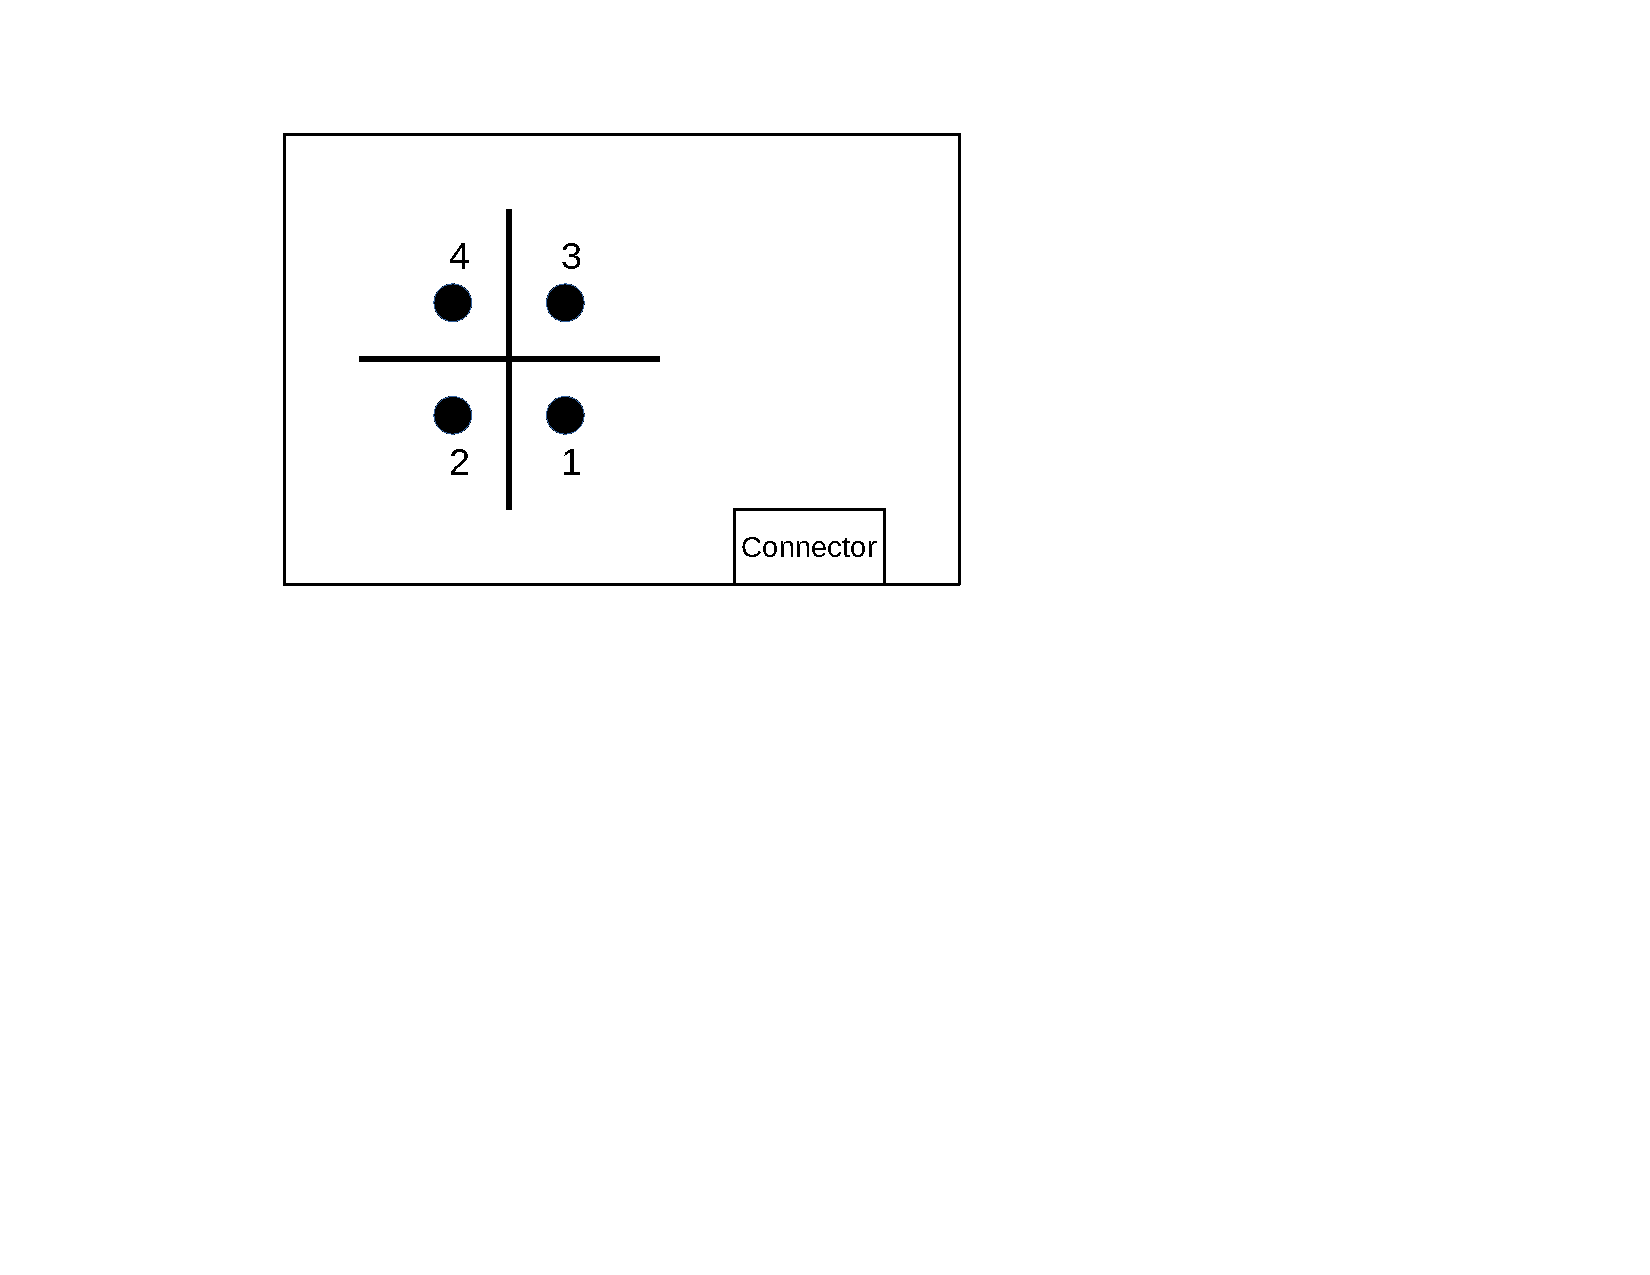
\includegraphics[scale=0.5]{Sensors.pdf}
    \caption{Light Sensor Arrangement}
    \label{fig:Sensors}
  \end{center}
\end{figure}

\subsection{Stepper Motor Control}
The stepper motors are controller by two TB6612 dual H-bridge controllers (Adafruit p/n 2448).  Each of these controls one of the stepper motors.  The first one, H1 is used to control the panning motor and the other one, H2 is used to control the tilt motor.

\subsection{Connections}
Both the controller and the pan tilt have two DB9 connectors (see figure \ref{fig:D9}).  One is used for the sensors (see table \ref{tbl:Sensor}) and the other is used for the stepper motors (see table \ref{tbl:Stepper}).

The cables are made using CAT5 cables and are wired up so that pins 1 \& 6, 2 \& 7, 4 \& 9, and 5 \& 9 are each on a separate twisted pair.  Which pair used is not particularly important, just that the pair is wired the same at both ends.

\begin{figure}[htb]
  \begin{center}
    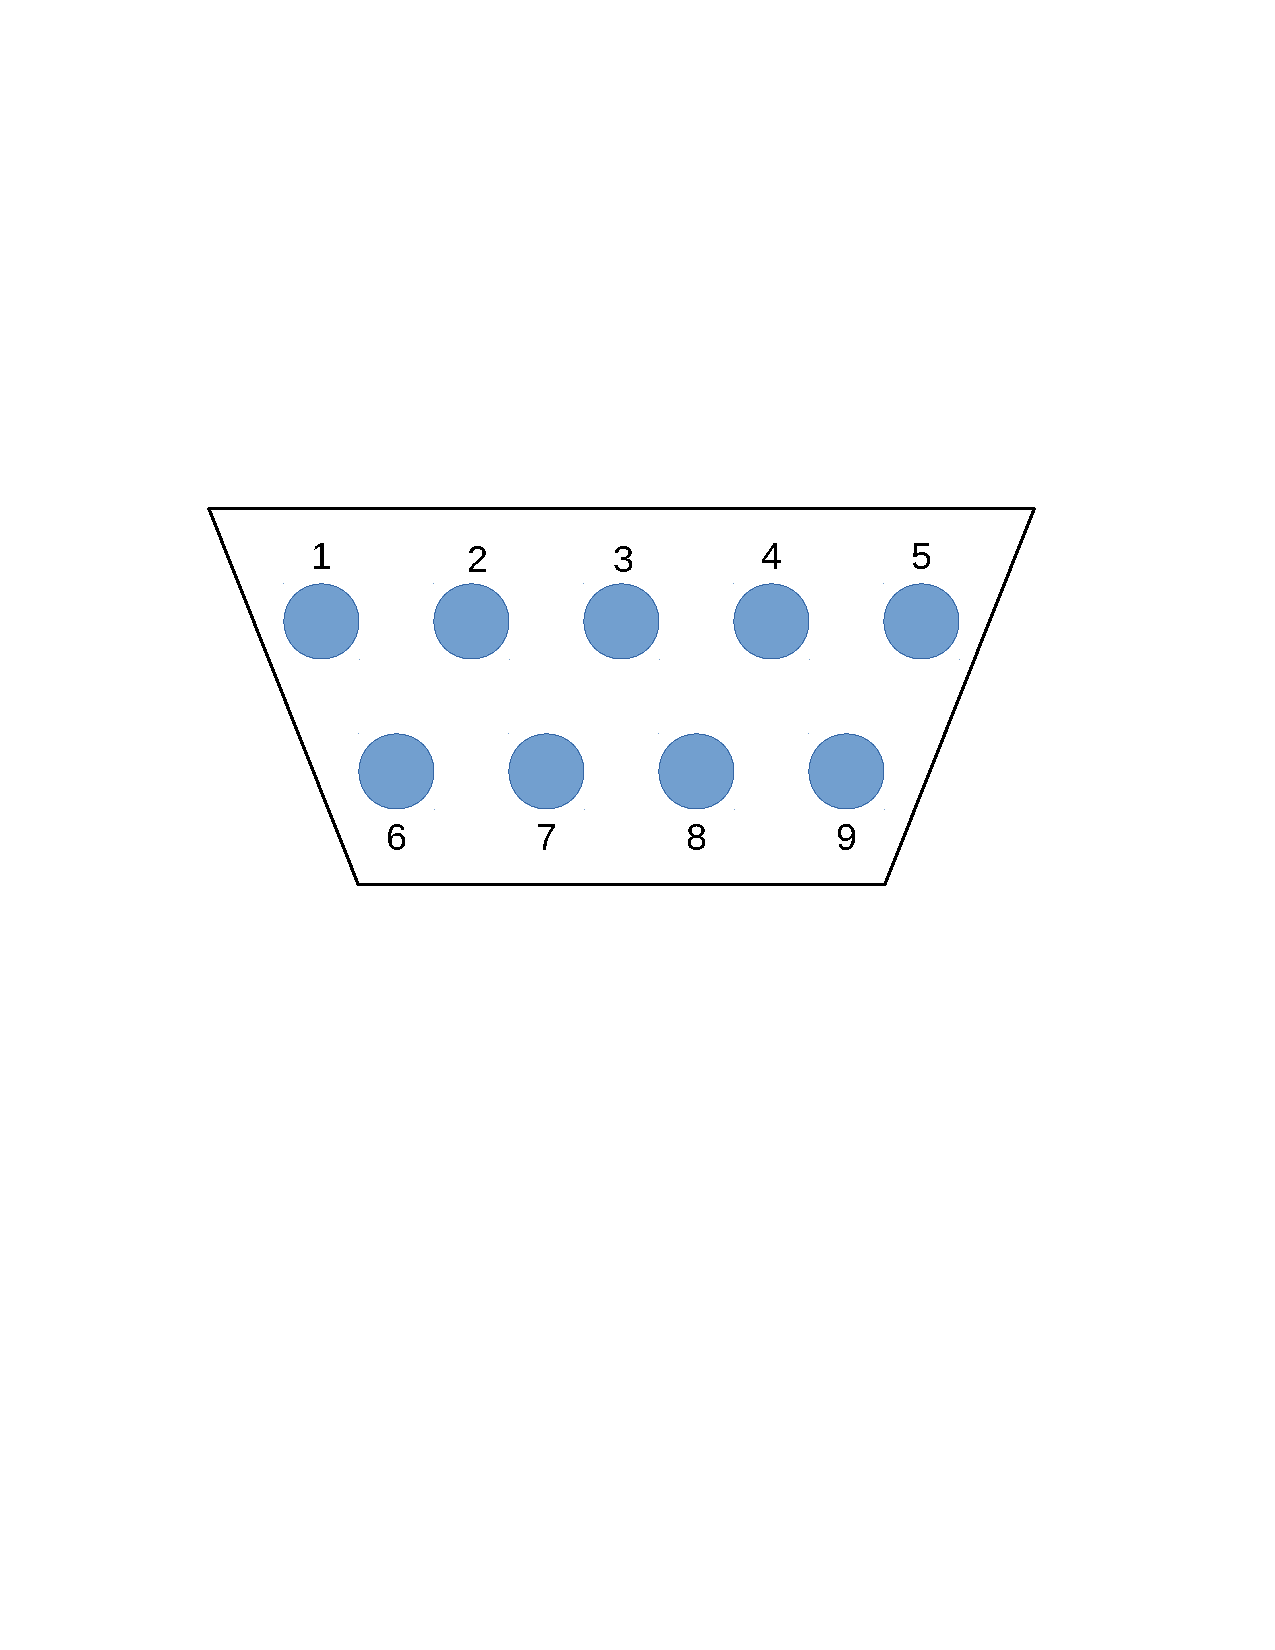
\includegraphics[scale=0.25]{D9Pins.pdf}
    \caption{DB-9 Connector Pin Numbers}
    \label{fig:D9}
  \end{center}
\end{figure}

\begin{table}
  \begin{center}
    \caption{Light Sensor Pinout}
    \label{tbl:Sensor}
    \begin{tabular}[htb]{|c|l|}
      \hline
      Pin & Usage \\
      \hline
      1 & Analog 4 \\
      2 & Analog 3 \\
      3 & n.c. \\
      4 & Analog 2 \\
      5 & Analog 1 \\
      6 & +V (for analog 4)\\
      7 & +V (for analog 3)\\
      8 & +V (for analog 2)\\
      9 & +V (for analog 1)\\
      \hline
    \end{tabular}
  \end{center}
\end{table}

\begin{table}
  \begin{center}
    \caption{Stepper Motor Connector Pinout}
    \label{tbl:Stepper}
    \begin{tabular}[htb]{|c|l|}
      \hline
      Pin & Usage \\
      \hline
      1 & H1, MA+ (gpio 22 green) \\
      2 & H1, MB+ (gpio 24 red) \\
      3 & n.c. \\
      4 & H2, MA+ (gpio 28 green) \\
      5 & H2, MB+ (gpio 30 red) \\
      6 & H1, MA- (gpio 23 grey) \\
      7 & H1, MB- (gpio 25 yellow) \\
      8 & H2, MA- (gpio 29 grey) \\
      9 & H2, MB- (gpio 31 yellow) \\
      \hline
    \end{tabular}
  \end{center}
\end{table}

\section{Mechanical}
\subsection{Gearing}
Both stepper motors have a 20 tooth gear and are 400 steps per revolution.

The tilt gear has 50 teeth giving a $\frac{2}{5}$ gear ratio.  With the gearing, 1000 steps of the motor will completely rotate the tilt frame.  This is 0.36\degree per step or 2.78 steps per degree.

The pan gear has 100 teeth giving a $\frac{1}{5}$ gear ratio.  With the gearing, 2000 steps of the motor will completely rotate the pan head, giving 0.18\degree per steps or 5.56 steps per degree.

\subsection{Control Box}

\subsection{Pan/Tilt Head}

%----------------------------------------------------------
\chapter{Software}

\end{document}

